\documentclass{article}

\usepackage{iclr2027_conference}

\usepackage[utf8]{inputenc}
\usepackage[T1]{fontenc}
\usepackage{hyperref}
\usepackage{url}
\usepackage{booktabs}
\usepackage{amsfonts}
\usepackage{amsmath}
\usepackage{mathtools}
\usepackage{amssymb}
\usepackage{amsthm}
\usepackage{nicefrac}
\usepackage{microtype}
\usepackage{xcolor}
\usepackage{graphicx}
\usepackage{float}
\usepackage{subcaption}
\usepackage{algorithm}
\usepackage{algorithmic}
\usepackage{wrapfig}
\usepackage{multirow}

\newtheorem{proposition}{Proposition}
\newtheorem{corollary}{Corollary}
\newtheorem{definition}{Definition}

\title{The Forecast--Reconstruction Tradeoff Is an Artifact\\of Coupling a Single Latent to Both Objectives}

\author{Arpit Goel \\
TwinSim Labs \\
\texttt{arpit@thebrownkid.in}}

\begin{document}

\maketitle

\begin{abstract}
Latent dynamical models that share a single latent space between
reconstruction and forecasting face a tradeoff: improving one
objective degrades the other.  We show this tradeoff is
architectural, not inherent.  For linear systems, we prove that
reconstruction-optimal and prediction-optimal projections
generically occupy different subspaces; empirically, we observe
persistent gradient conflict on the shared encoder.
We propose \emph{carrier-residual decoupling}: a wide carrier
handles reconstruction, a narrow residual code handles forecasting,
and no parameters are shared between the two.
On five dynamical systems (6--20D), a 64D spatiotemporal benchmark,
three forecast heads (DMD, MLP, neural ODE), and four multi-task
gradient methods, no param-matched coupled model Pareto-dominates
the decoupled one.
\end{abstract}


% ======================================================================
\section{Introduction}
\label{sec:intro}

Autoencoder-based latent dynamical models learn a low-dimensional
representation of high-dimensional observations and fit a dynamics
model in that latent space.  The representation must simultaneously
preserve enough variance for faithful reconstruction and exhibit
temporal regularity that the dynamics model can exploit.  These two
requirements compete: the standard weighted loss
$\mathcal{L} = (1{-}\varphi)\,\mathcal{L}_{\mathrm{rec}} +
\varphi\,\mathcal{L}_{\mathrm{fcst}}$
traces a Pareto frontier as $\varphi$ varies, and no single setting
minimises both~\citep{lusch2018deep,otto2019linearly}.

This tradeoff is widely accepted.  We argue it reflects a limitation
of the \emph{coupled} architecture---one encoder, one latent, two
objectives---rather than a fundamental property of the learning
problem.  Two arguments support this claim:
\begin{enumerate}
\item \textbf{Capacity bound.}  The rank-$k$ projection that
minimises reconstruction error captures the top-$k$ variance
directions, while the projection that minimises prediction error
captures the top-$k$ \emph{predictable} directions.
For a linear system these are the eigenvectors of two different
matrices ($\Sigma_x$ vs.\ $F\Sigma_x F^\top$), which generically
do not align (Proposition~\ref{prop:capacity}).  For nonlinear
systems the mismatch is strictly worse, because the relevant
Jacobian varies across the state space
(Corollary~\ref{cor:nonlinear}).
\item \textbf{Gradient conflict.}  The gradients of reconstruction
and forecasting losses on the shared encoder point in opposing
directions 62--92\% of training batches, so each gradient step
compromises at least one objective
(Section~\ref{sec:gradient-conflict}).
\end{enumerate}
If the bottleneck is architectural, then allocating separate subspaces
to each objective should remove it.  We propose \emph{carrier-residual
decoupling}: a wide $j$-dim carrier optimised for reconstruction,
and a narrow $k$-dim residual code optimised for dynamics, trained
in three frozen-teacher phases with no shared gradient path.

We evaluate on five synthetic systems (6--20D) plus
Kuramoto--Sivashinsky (64D), across three forecast heads (DMD, MLP,
neural ODE), four multi-task gradient methods (PCGrad, CAGrad,
Nash-MTL, FAMO), and three literature methods (mLaSDI, Koopa, AIKAE).
All baselines are parameter-matched.  The decoupled model
achieves lower reconstruction and forecast error in the large
majority of comparisons where a single model must serve both
objectives.


% ======================================================================
\section{Background}
\label{sec:background}

\paragraph{Koopman autoencoders and DMD.}
The Koopman operator~\citep{koopman1931hamiltonian,mezic2005spectral}
lifts nonlinear dynamics into a linear, infinite-dimensional
representation.  Deep autoencoders learn finite-dimensional
approximations: the encoder maps observations to coordinates where
dynamics are approximately linear, and the decoder maps
back~\citep{lusch2018deep,takeishi2017learning,otto2019linearly,
yeung2019learning,champion2019data,gin2021deep}.
Physics-informed~\citep{erichson2019,pan2020physics} and
consistent~\citep{azencot2020} variants add stability penalties;
AIKAE~\citep{li2022deep} adds auxiliary-task invariant subspaces;
Koopa~\citep{liu2024koopa} learns the operator end-to-end.
All retain the coupled architecture.
Dynamic Mode Decomposition (DMD)~\citep{schmid2010dmd} fits a
best-fit linear operator $A = Y X^\dagger$; its eigendecomposition
$A = V\Lambda V^{-1}$ enables non-iterative multi-step prediction
$z_{T+\tau} = V\Lambda^\tau V^{-1} z_T$~\citep{brunton2022modern}.
mLaSDI~\citep{bonneville2024mlasdi} stacks multiple latent-space
DMD models for parametric problems.

\paragraph{Multi-task learning.}
Joint training of reconstruction and forecasting is multi-task
learning~\citep{sener2018multi}.  When task gradients conflict,
PCGrad~\citep{yu2020gradient} projects out the conflicting component,
CAGrad~\citep{liu2021conflict} finds a common descent direction,
Nash-MTL~\citep{navon2022multi} frames the problem as a bargaining
game, and FAMO~\citep{liu2024famo} adapts task weights online.
All four methods modify the training procedure to mitigate gradient
interference; none changes the underlying shared-encoder architecture.

\paragraph{Residual learning and neural ODEs.}
Residual connections~\citep{he2016deep} decompose a function into an
identity plus a learned residual; our carrier-residual decomposition
applies the same idea temporally.
Neural ODEs~\citep{chen2018neural,rubanova2019latent} parameterise
continuous-time dynamics $dz/dt = f_\theta(z)$; we use them as one of
three pluggable forecast heads.


% ======================================================================
\section{Theory}
\label{sec:theory}

\subsection{Capacity Bound}
\label{sec:capacity-bound}

Consider a linear system
$\mathbf{x}_{t+1} = F\,\mathbf{x}_t + \boldsymbol{\varepsilon}_t$,
$\boldsymbol{\varepsilon}_t \sim \mathcal{N}(\mathbf{0}, Q)$,
with stationary covariance $\Sigma_x = F\Sigma_x F^\top + Q$.
We seek an orthonormal $P \in \mathbb{R}^{n \times k}$,
$\Pi = PP^\top$.
The reconstruction loss
$\mathcal{L}_{\mathrm{rec}}(P)
= \mathrm{tr}(\Sigma_x) - \mathrm{tr}(P^\top\Sigma_x P)$
is minimised by the top-$k$ eigenvectors of $\Sigma_x$.
The prediction loss
$\mathcal{L}_{\mathrm{pred}}(P)
= \mathrm{tr}(M^\top M \Sigma_x) + \mathrm{tr}(Q)$,
$M = F - \Pi F \Pi$, captures the dynamics approximation error.

\begin{proposition}[Capacity bound]
\label{prop:capacity}
Let $\Sigma_x$ have distinct eigenvalues.
If $F\Sigma_x \neq \Sigma_x F$, then the reconstruction-optimal
projection $P_{\mathrm{rec}}^*$ is not a stationary point of the
prediction loss, and no single rank-$k$ projection simultaneously
minimises both objectives.
\end{proposition}

\begin{proof}
Consider $n{=}2$, $k{=}1$, $\Sigma_x = \mathrm{diag}(\lambda_1, \lambda_2)$
with $\lambda_1 > \lambda_2 > 0$, so $P_{\mathrm{rec}}^* = e_1$.

At $P = e_1$:
$\mathcal{L}_{\mathrm{pred}}(e_1) = \lambda_1 F_{21}^2 + \lambda_2 F_{12}^2 + \lambda_2 F_{22}^2 + \mathrm{tr}(Q)$.

At $P = e_2$:
$\mathcal{L}_{\mathrm{pred}}(e_2) = \lambda_1 F_{11}^2 + \lambda_2 F_{12}^2 + \mathrm{tr}(Q)$.

The reconstruction-optimal $e_1$ is prediction-optimal only when
$\lambda_1 F_{21}^2 + \lambda_2 F_{22}^2 \le \lambda_1 F_{11}^2$.
This fails whenever the off-diagonal or lower-right entries of $F$
are sufficiently large---the generic case when
$F\Sigma_x \neq \Sigma_x F$.

For general $n,k$: replacing $v_k$ with $v_{k+1}$ in $P$ increases
$\mathcal{L}_{\mathrm{rec}}$ by $\lambda_k - \lambda_{k+1} > 0$ but
can decrease $\mathcal{L}_{\mathrm{pred}}$ whenever $F$ couples the
retained and excluded eigenspaces.  This coupling is absent only when
$F$ and $\Sigma_x$ commute (measure zero).
\end{proof}

\begin{corollary}[Nonlinear extension]
\label{cor:nonlinear}
Let $\mathbf{x}_{t+1} = f(\mathbf{x}_t) + \boldsymbol{\varepsilon}_t$
with differentiable $f$ and Jacobian
$J(\mathbf{x}) = \nabla f(\mathbf{x})$.
If $J$ is not constant on the support of the data distribution
(i.e.\ the dynamics are genuinely nonlinear), then the capacity
bound is strictly tighter than in the linear case: no single
rank-$k$ projection can simultaneously minimise reconstruction
and prediction error.
\end{corollary}

\begin{proof}
At each state $\mathbf{x}_0$, one-step prediction through a rank-$k$
projection $P$ incurs a local error governed by the Jacobian
$J(\mathbf{x}_0)$, which plays the role of $F$ in
Proposition~\ref{prop:capacity}.
The locally prediction-optimal projection therefore depends on
$J(\mathbf{x}_0)$.
When $J$ varies across the attractor---as it does for any
genuinely nonlinear system---the locally optimal $P$ varies with it.

A global encoder must fix a single $P$.  By
Proposition~\ref{prop:capacity}, at any state where
$J(\mathbf{x}_0)\Sigma_x \neq \Sigma_x J(\mathbf{x}_0)$,
the reconstruction-optimal $P$ is not locally prediction-optimal.
Since $J$ is non-constant, this condition holds
on an open dense subset of the attractor.
Thus the capacity constraint is at least as strong as in the
constant-$J$ (linear) case, and strictly stronger when $J$
varies sufficiently.
\end{proof}

\paragraph{Implication.}
The capacity bound applies to all five benchmark systems: directly
for the linear system (Linear 5D) and via
Corollary~\ref{cor:nonlinear} for the nonlinear ones
(Coupled Harmonic, Brusselator, Duffing, Lorenz-96).
Carrier-residual decoupling avoids this constraint: $j$ dimensions
serve reconstruction and $k$ dimensions serve dynamics, so neither
is forced into a compromise projection.


\subsection{Gradient Conflict}
\label{sec:gradient-conflict}

\begin{proposition}[Gradient conflict]
\label{prop:gradient-conflict}
In a coupled autoencoder with loss
$(1{-}\varphi)\mathcal{L}_{\mathrm{rec}} +
\varphi\mathcal{L}_{\mathrm{fcst}}$,
let $\mathbf{g}_r$ and $\mathbf{g}_f$ be the gradients of the two
losses w.r.t.\ the shared encoder.  If
$\langle \mathbf{g}_r, \mathbf{g}_f \rangle < 0$, then for any
$\varphi \in (0,1)$: \emph{(a)} the combined gradient makes less
progress on each objective than the individual gradient would;
\emph{(b)} gradient magnitude is reduced by inter-task cancellation;
\emph{(c)} extreme $\varphi$ values actively increase the opposing
objective.
In the decoupled architecture, $\mathbf{g}_f = \mathbf{0}$ on the
encoder and no conflict arises.
\end{proposition}

\begin{proof}
Let $\mathbf{g}_\varphi = (1{-}\varphi)\mathbf{g}_r + \varphi\mathbf{g}_f$.

\emph{(a)}
$\langle \mathbf{g}_\varphi, \mathbf{g}_r \rangle
= (1{-}\varphi)\|\mathbf{g}_r\|^2 + \varphi\langle\mathbf{g}_f,\mathbf{g}_r\rangle$.
Since $\varphi > 0$ and
$\langle\mathbf{g}_f,\mathbf{g}_r\rangle < 0$,
this is strictly less than $\|\mathbf{g}_r\|^2$.
Symmetric for $\mathbf{g}_f$.

\emph{(b)}
$\|\mathbf{g}_\varphi\|^2
= (1{-}\varphi)^2\|\mathbf{g}_r\|^2
+ 2\varphi(1{-}\varphi)\langle\mathbf{g}_r,\mathbf{g}_f\rangle
+ \varphi^2\|\mathbf{g}_f\|^2$.
The cross-term is negative.

\emph{(c)}
$\langle\mathbf{g}_\varphi,\mathbf{g}_r\rangle < 0$
iff $\varphi > \|\mathbf{g}_r\|^2
/ (\|\mathbf{g}_r\|^2 + |\langle\mathbf{g}_f,\mathbf{g}_r\rangle|)
\eqqcolon \varphi_{\mathrm{hi}}$.
By Cauchy--Schwarz, $\varphi_{\mathrm{hi}} \in (0,1)$.
The threshold $\varphi_{\mathrm{lo}}$ for
$\langle\mathbf{g}_\varphi,\mathbf{g}_f\rangle < 0$ is analogous,
and $\varphi_{\mathrm{lo}} < \varphi_{\mathrm{hi}}$.
\end{proof}


\paragraph{Empirical verification.}
We train coupled autoencoders at six $\varphi$ values and log
$\cos(\mathbf{g}_r, \mathbf{g}_f)$ on the encoder every 10 batches.
Figure~\ref{fig:gradient-conflict} shows the cosine is negative
62--92\% of the time across all systems, with mean cosine between
$-0.23$ and $-0.03$.  The conflict persists throughout training.

\begin{figure}[H]
\centering
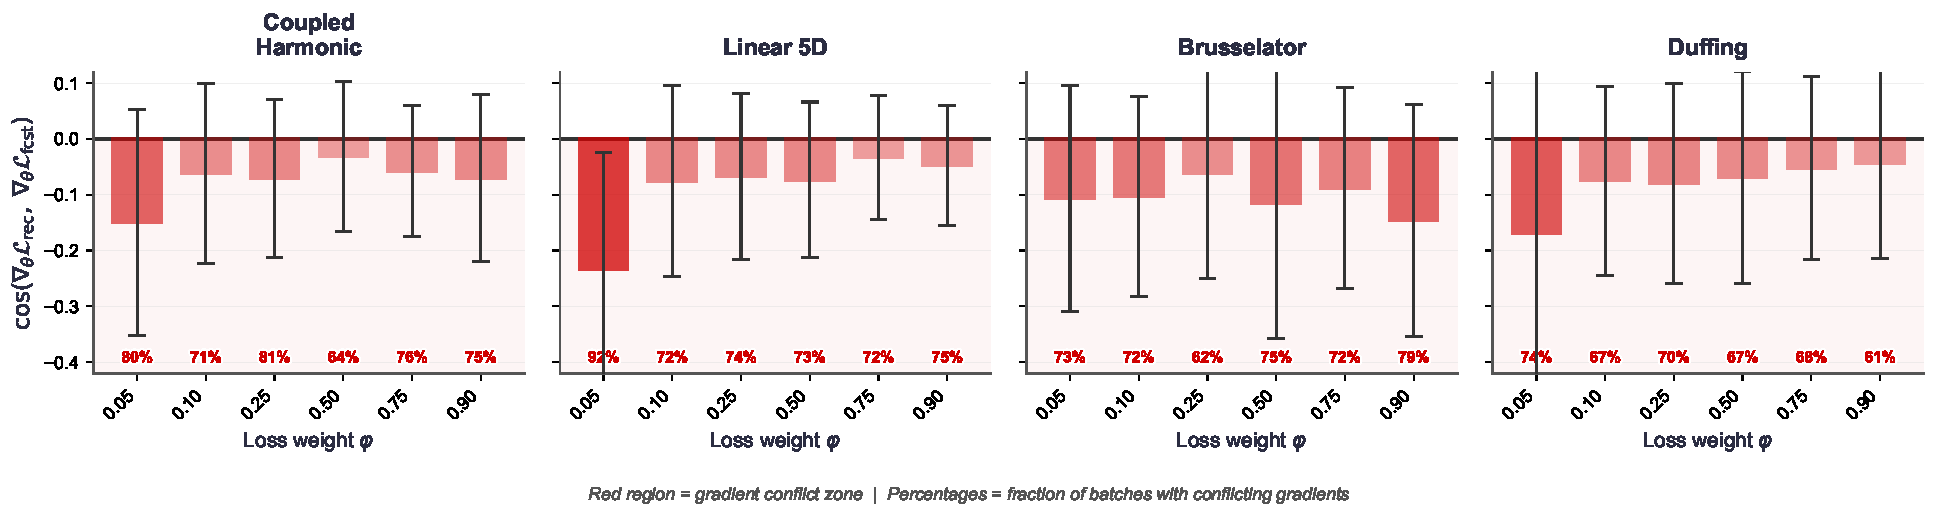
\includegraphics[width=\textwidth]{gradient_conflict.png}
\caption{Cosine similarity between reconstruction and forecasting
gradients on the shared encoder.  Red bars: negative mean cosine.
Percentages: fraction of batches with conflict.}
\label{fig:gradient-conflict}
\end{figure}


% ======================================================================
\section{Method}
\label{sec:method}

The core idea is to decouple a latent dynamical model into two
non-overlapping subspaces: a \emph{reconstruction subspace} of
dimension $j$, optimised solely for observation fidelity, and a
\emph{dynamics subspace} of dimension $k \ll j$, optimised solely for
temporal prediction.  No parameters are shared between the two after
the reconstruction module is trained, so neither objective's gradient
can interfere with the other.
Any encoder--decoder pair, any dynamics model, and any accumulation
rule can fill these roles; the principle defines a family of
\emph{decoupled latent dynamical models}.  Below we describe one
concrete instantiation: a three-phase frozen-teacher pipeline.

\paragraph{Phase 1: Teacher autoencoder.}
An encoder $E: \mathbb{R}^n \to \mathbb{R}^j$ and decoder
$D: \mathbb{R}^j \to \mathbb{R}^n$ are trained for reconstruction.
The carrier $C_t = E(x_t)$ is wide enough ($j > k$) for near-perfect
reconstruction.

\paragraph{Phase 2: Residual compressor.}
With $E,D$ frozen, carrier residuals $\Delta C_t = C_{t+1} - C_t$ are
compressed:
$\psi: \mathbb{R}^j \to \mathbb{R}^k$,
$\mu: \mathbb{R}^k \to \mathbb{R}^j$,
trained to minimise
$\|\Delta C_t - \mu(\psi(\Delta C_t))\|^2$.
The residual code $b_t = \psi(\Delta C_t) \in \mathbb{R}^k$ captures
temporal dynamics in a form amenable to prediction.

\paragraph{Phase 3: GRU accumulation.}
During forecasting, the carrier evolves via gated accumulation:
$C_{t+1} = \mathrm{GRU}(\mu(b_t), C_t)$,
trained with all prior modules frozen.  This replaces naive addition
$C_{t+1} = C_t + \mu(b_t)$, which compounds errors over long rollouts.

\paragraph{Pluggable forecast heads.}
\label{sec:heads}
Any model predicting $b_{t+1}$ from $b_t$ serves as the forecast
head.  We test three: \textbf{DMD} (post-hoc linear,
$b_{t+1} = Ab_t$), \textbf{MLP} (learned nonlinear), and
\textbf{neural ODE} ($db/dt = f_\theta(b)$, RK4 integration).
All share the same frozen teacher, so reconstruction is identical
across heads.


% ======================================================================
\section{Experiments}
\label{sec:experiments}

\subsection{Setup}

\paragraph{Systems.}
Five synthetic dynamical systems: Coupled Harmonic Oscillator
(6D), Linear 5D, Brusselator (10D), forced Duffing
(10D), and Lorenz-96 (20D).  We additionally test
Kuramoto--Sivashinsky (KS, 64D) for scalability.

\paragraph{Protocol.}
Carrier $j{=}8$ (systems $\le$10D), $j{=}12$ (L-96), $j{=}32$
(KS-64D); residual $k$ matches the coupled AE latent dim.
All models: 400 epochs/phase, batch 512, Adam ($10^{-3}$).
The decoupled model uses hidden width $h{=}64$; each coupled
baseline's $h$ is widened ($h{\approx}73$--$95$) until its total
parameter count meets or exceeds the decoupled model's
($1.00$--$1.01\times$; Appendix~\ref{app:params}).
Results: mean over 5 seeds.

\paragraph{Metrics.}
Reconstruction RMSE (R) and forecast RMSE at horizon $\tau$ (F$\tau$).
For coupled DMD baselines and all decoupled variants, forecast uses
spectral DMD ($z_{T+\tau} = V\Lambda^\tau V^{-1} z_T$).
For coupled MLP and ODE heads, forecast uses each head's own
learned predictor.

\paragraph{Baselines.}
\emph{Coupled}: AE trained with
$(1{-}\varphi)\mathcal{L}_{\mathrm{rec}} +
\varphi\mathcal{L}_{\mathrm{fcst}}$ at $\varphi{=}0.5$.
\emph{Decoupled}: carrier-residual architecture above.


\subsection{Head Comparison}
\label{sec:head-comparison}

Does decoupling help regardless of how the dynamics are modelled?
Table~\ref{tab:head-comparison} pairs each coupled head (DMD,
MLP, neural ODE) against the decoupled model.  Each coupled model
is param-matched and trained jointly at $\varphi{=}0.5$; each uses
its own head for prediction.

The Decoupled columns are identical across rows because the
reconstruction comes entirely from the frozen Phase~1 teacher and the
forecast is evaluated via spectral DMD on the same frozen $b$
trajectory, irrespective of which head was trained in Phase~2.5.
On four of five systems, Decoupled achieves lower R \emph{and}
lower F1 than every coupled head.  On Brusselator, the coupled ODE
achieves F1$=$\,.005 (vs.\ Decoupled~.013) at the cost of
R$=$\,.005 (vs.\ Decoupled~.002): exactly the tradeoff the capacity
bound predicts.

\begin{table}[H]
\caption{Head comparison (mean$\pm$std, 5 seeds).
Coupled models are param-matched ($h{=}73$--$76$).
Decoupled values are identical across heads: reconstruction depends
only on the frozen teacher; forecast uses spectral DMD on the same
frozen $b$ trajectory (\S\ref{sec:heads}).
\textbf{Bold}: best per row.}
\label{tab:head-comparison}
\centering
\small
\setlength{\tabcolsep}{3pt}
\begin{tabular}{l l cc cc}
\toprule
& & \multicolumn{2}{c}{Coupled} & \multicolumn{2}{c}{Decoupled} \\
\cmidrule(lr){3-4}\cmidrule(lr){5-6}
System & Head & R & F1 & R & F1 \\
\midrule
\multirow{3}{*}{C.~Harm.}
  & DMD & $.702{\scriptstyle\pm.092}$ & $.815{\scriptstyle\pm.056}$
  & $\mathbf{.006}{\scriptstyle\pm.000}$ & $\mathbf{.012}{\scriptstyle\pm.000}$ \\
  & MLP & $.221{\scriptstyle\pm.070}$ & $.218{\scriptstyle\pm.068}$
  & $\mathbf{.006}{\scriptstyle\pm.000}$ & $\mathbf{.012}{\scriptstyle\pm.000}$ \\
  & ODE & $.340{\scriptstyle\pm.042}$ & $.338{\scriptstyle\pm.041}$
  & $\mathbf{.006}{\scriptstyle\pm.000}$ & $\mathbf{.012}{\scriptstyle\pm.000}$ \\
\addlinespace
\multirow{3}{*}{Lin.~5D}
  & DMD & $.563{\scriptstyle\pm.110}$ & $.679{\scriptstyle\pm.115}$
  & $\mathbf{.005}{\scriptstyle\pm.001}$ & $\mathbf{.005}{\scriptstyle\pm.001}$ \\
  & MLP & $.013{\scriptstyle\pm.001}$ & $.014{\scriptstyle\pm.001}$
  & $\mathbf{.005}{\scriptstyle\pm.001}$ & $\mathbf{.005}{\scriptstyle\pm.001}$ \\
  & ODE & $.009{\scriptstyle\pm.001}$ & $.009{\scriptstyle\pm.001}$
  & $\mathbf{.005}{\scriptstyle\pm.001}$ & $\mathbf{.005}{\scriptstyle\pm.001}$ \\
\addlinespace
\multirow{3}{*}{Bruss.}
  & DMD & $.479{\scriptstyle\pm.267}$ & $.665{\scriptstyle\pm.263}$
  & $\mathbf{.002}{\scriptstyle\pm.000}$ & $\mathbf{.013}{\scriptstyle\pm.001}$ \\
  & MLP & $.027{\scriptstyle\pm.012}$ & $.026{\scriptstyle\pm.013}$
  & $\mathbf{.002}{\scriptstyle\pm.000}$ & $\mathbf{.013}{\scriptstyle\pm.001}$ \\
  & ODE & $.005{\scriptstyle\pm.002}$ & $\mathbf{.005}{\scriptstyle\pm.002}$
  & $\mathbf{.002}{\scriptstyle\pm.000}$ & $.013{\scriptstyle\pm.001}$ \\
\addlinespace
\multirow{3}{*}{Duffing}
  & DMD & $.577{\scriptstyle\pm.251}$ & $.589{\scriptstyle\pm.153}$
  & $\mathbf{.005}{\scriptstyle\pm.001}$ & $\mathbf{.006}{\scriptstyle\pm.001}$ \\
  & MLP & $.017{\scriptstyle\pm.015}$ & $.015{\scriptstyle\pm.016}$
  & $\mathbf{.005}{\scriptstyle\pm.001}$ & $\mathbf{.006}{\scriptstyle\pm.001}$ \\
  & ODE & $.009{\scriptstyle\pm.004}$ & $.008{\scriptstyle\pm.004}$
  & $\mathbf{.005}{\scriptstyle\pm.001}$ & $\mathbf{.006}{\scriptstyle\pm.001}$ \\
\addlinespace
\multirow{3}{*}{L-96}
  & DMD & $.740{\scriptstyle\pm.035}$ & $.810{\scriptstyle\pm.053}$
  & $\mathbf{.387}{\scriptstyle\pm.007}$ & $\mathbf{.406}{\scriptstyle\pm.007}$ \\
  & MLP & $.600{\scriptstyle\pm.009}$ & $.577{\scriptstyle\pm.006}$
  & $\mathbf{.387}{\scriptstyle\pm.007}$ & $\mathbf{.406}{\scriptstyle\pm.007}$ \\
  & ODE & $.598{\scriptstyle\pm.015}$ & $.574{\scriptstyle\pm.009}$
  & $\mathbf{.387}{\scriptstyle\pm.007}$ & $\mathbf{.406}{\scriptstyle\pm.007}$ \\
\bottomrule
\end{tabular}
\end{table}


\subsection{Scalability: KS-64D}
\label{sec:highdim}

To test whether the advantage holds in higher dimensions, we evaluate
on Kuramoto--Sivashinsky with $n{=}64$ spatial modes
(Table~\ref{tab:ks}).  The decoupled model ($j{=}32$, $k{=}16$,
$h{=}64$, 33\,488 params) is compared against a param-matched
coupled baseline ($k{=}16$, $h{=}95$, 33\,966 params).
Decoupled achieves 6$\times$ lower reconstruction error and lower
forecast error at every horizon.

\begin{table}[H]
\caption{KS-64D (mean$\pm$std, 5 seeds).
Coupled is param-matched ($h{=}95$, 33\,966 params).}
\label{tab:ks}
\centering
\small
\begin{tabular}{l rrrrr}
\toprule
Method & R & F1 & F10 & F50 & F100 \\
\midrule
Coupled & $.378{\scriptstyle\pm.017}$ & $.363{\scriptstyle\pm.064}$
  & $.810{\scriptstyle\pm.073}$ & $1.05{\scriptstyle\pm.05}$
  & $1.10{\scriptstyle\pm.07}$ \\
Decoupled & $\mathbf{.062}{\scriptstyle\pm.003}$ & $\mathbf{.050}{\scriptstyle\pm.002}$
  & $\mathbf{.166}{\scriptstyle\pm.010}$ & $\mathbf{.646}{\scriptstyle\pm.076}$
  & $\mathbf{.926}{\scriptstyle\pm.08}$ \\
\bottomrule
\end{tabular}
\end{table}


\subsection{Ablation}
\label{sec:ablation}

What drives the improvement?  Table~\ref{tab:ablation} isolates each
component.
\emph{Coupled\_k}: param-matched $k$-dim AE + spectral DMD.
\emph{Coupled\_j}: $j$-dim AE (wider latent, more capacity).
\emph{Frozen\_j}: $j$-dim AE trained recon-only, spectral DMD
applied post-hoc (no dynamics gradient on the encoder).
\emph{Frozen\_k}: same but $k$-dim.
\emph{Decoupled}: full carrier-residual + spectral DMD.

Frozen\_j achieves the lowest reconstruction error---it has the
widest latent and no dynamics gradient to distort it---but it provides
no dynamics pipeline for multi-step rollout.
Frozen\_k has the dynamics bottleneck but poor reconstruction.
Decoupled matches Frozen\_j on reconstruction while providing the
residual code pathway for forecasting.  No single baseline achieves
both; Decoupled does.

\begin{table}[H]
\caption{Ablation (mean, 5 seeds).
Coupled\_k is param-matched ($h{=}73$--$76$).
\textbf{Bold}: best in each row.}
\label{tab:ablation}
\centering
\small
\setlength{\tabcolsep}{3pt}
\begin{tabular}{l cc cc cc cc cc}
\toprule
& \multicolumn{2}{c}{Coupled\_k} & \multicolumn{2}{c}{Coupled\_j}
& \multicolumn{2}{c}{Frozen\_j} & \multicolumn{2}{c}{Frozen\_k}
& \multicolumn{2}{c}{Decoupled} \\
\cmidrule(lr){2-3}\cmidrule(lr){4-5}\cmidrule(lr){6-7}\cmidrule(lr){8-9}\cmidrule(lr){10-11}
System & R & F1 & R & F1 & R & F1 & R & F1 & R & F1 \\
\midrule
C.~Harm.
  & .702 & .815
  & .032 & .032
  & $\mathbf{.006}$ & $\mathbf{.008}$
  & .167 & .169
  & $\mathbf{.006}$ & .012 \\
Lin.~5D
  & .563 & .679
  & $\mathbf{.005}$ & .007
  & $\mathbf{.005}$ & .006
  & .011 & .035
  & $\mathbf{.005}$ & $\mathbf{.005}$ \\
Bruss.
  & .479 & .665
  & $\mathbf{.002}$ & $\mathbf{.007}$
  & $\mathbf{.002}$ & $\mathbf{.007}$
  & $\mathbf{.002}$ & .048
  & $\mathbf{.002}$ & .013 \\
Duffing
  & .577 & .589
  & $\mathbf{.004}$ & $\mathbf{.005}$
  & $\mathbf{.004}$ & $\mathbf{.005}$
  & .009 & .031
  & .005 & .006 \\
L-96
  & .740 & .810
  & .401 & .422
  & .401 & .422
  & .523 & .541
  & $\mathbf{.387}$ & $\mathbf{.406}$ \\
\bottomrule
\end{tabular}
\end{table}


\subsection{Multi-Task Gradient Methods}
\label{sec:mtl}

If the problem is solely gradient conflict, perhaps better
optimisation can fix the coupled model.  We test four multi-task methods---PCGrad,
CAGrad, Nash-MTL, FAMO---against the naive weighted sum
(Table~\ref{tab:mtl}).  All coupled models are param-matched.
None substantially improves over the naive baseline; all remain
far from the decoupled result.  The bottleneck is architectural,
not optimisation-level.

\begin{table}[H]
\caption{Multi-task methods vs.\ Decoupled: F1 RMSE (mean$\pm$std, 5 seeds).
All coupled models param-matched ($h{=}73$--$76$).}
\label{tab:mtl}
\centering
\small
\setlength{\tabcolsep}{2.5pt}
\begin{tabular}{l cccccc}
\toprule
System & Naive & \shortstack{PCGrad\\\citep{yu2020gradient}} & \shortstack{CAGrad\\\citep{liu2021conflict}} & \shortstack{Nash-MTL\\\citep{navon2022multi}} & \shortstack{FAMO\\\citep{liu2024famo}} & Decoupled \\
\midrule
C.~Harm.
  & $.815{\scriptstyle\pm.056}$
  & $.754{\scriptstyle\pm.084}$
  & $.893{\scriptstyle\pm.146}$
  & $.774{\scriptstyle\pm.051}$
  & $.723{\scriptstyle\pm.070}$
  & $\mathbf{.012}{\scriptstyle\pm.000}$ \\
Lin.~5D
  & $.679{\scriptstyle\pm.115}$
  & $.562{\scriptstyle\pm.093}$
  & $.654{\scriptstyle\pm.167}$
  & $.581{\scriptstyle\pm.101}$
  & $.607{\scriptstyle\pm.156}$
  & $\mathbf{.005}{\scriptstyle\pm.001}$ \\
Bruss.
  & $.665{\scriptstyle\pm.263}$
  & $.417{\scriptstyle\pm.115}$
  & $.560{\scriptstyle\pm.217}$
  & $.577{\scriptstyle\pm.181}$
  & $.878{\scriptstyle\pm.817}$
  & $\mathbf{.013}{\scriptstyle\pm.001}$ \\
Duffing
  & $.589{\scriptstyle\pm.153}$
  & $.660{\scriptstyle\pm.180}$
  & $.712{\scriptstyle\pm.451}$
  & $.815{\scriptstyle\pm.529}$
  & $.383{\scriptstyle\pm.188}$
  & $\mathbf{.006}{\scriptstyle\pm.001}$ \\
L-96
  & $.810{\scriptstyle\pm.053}$
  & $.789{\scriptstyle\pm.044}$
  & $.585{\scriptstyle\pm.031}$
  & $.776{\scriptstyle\pm.026}$
  & $.799{\scriptstyle\pm.022}$
  & $\mathbf{.406}{\scriptstyle\pm.007}$ \\
\bottomrule
\end{tabular}
\end{table}


\subsection{Pareto Frontier}
\label{sec:pareto}

Figure~\ref{fig:frontier} shows the full picture.  Sweeping
$\varphi \in \{0, 0.05, \dots, 1\}$ traces a Pareto frontier for
the coupled model (grey).  The decoupled model
(\textcolor{red}{$\star$}) falls inside this frontier on all five
systems: it achieves near-$\varphi{=}0$ reconstruction with
comparable or better forecast quality.

\begin{figure}[H]
\centering
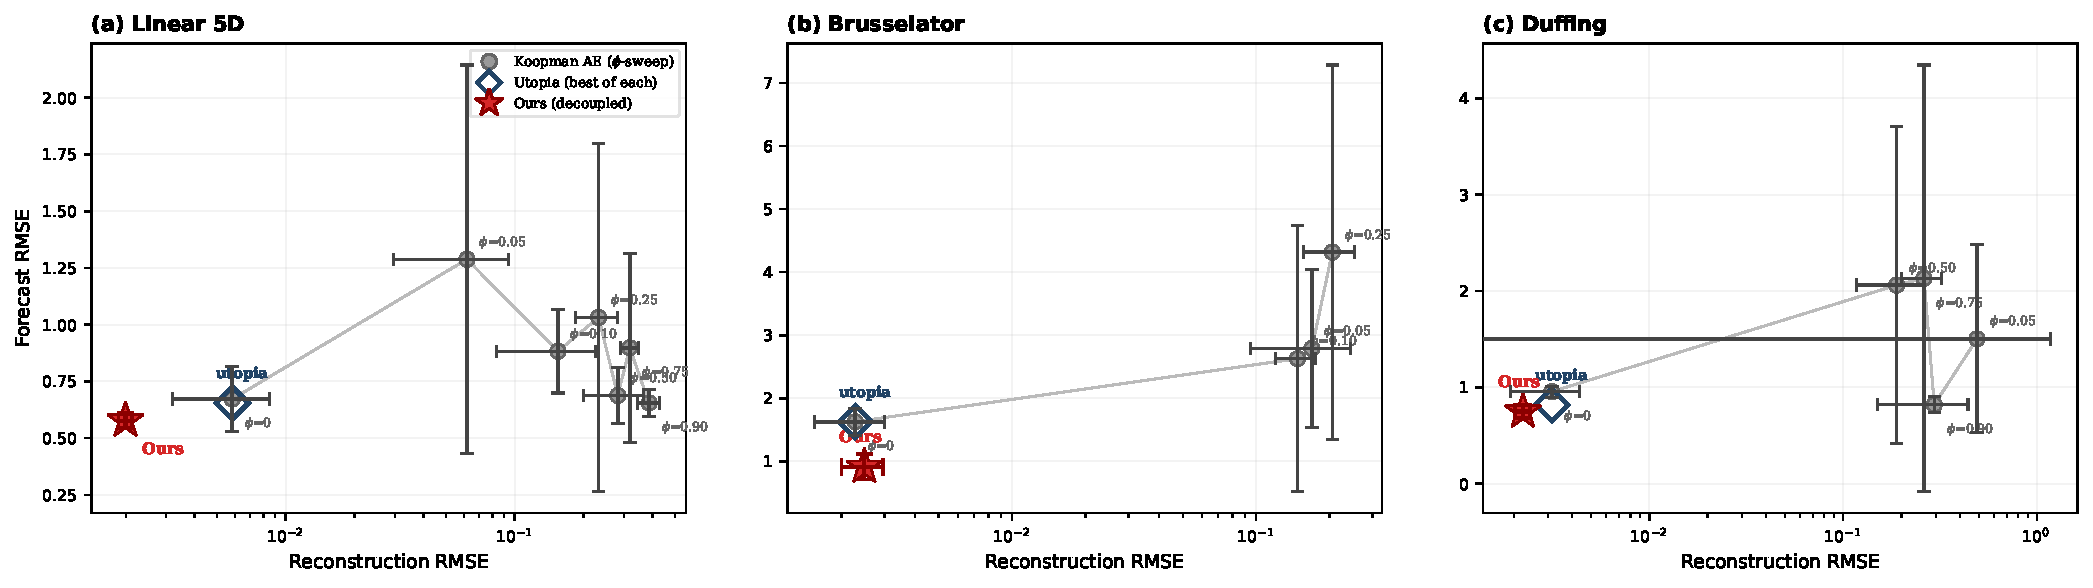
\includegraphics[width=\textwidth]{phi_sweep.png}
\caption{$\varphi$-sweep Pareto frontier (grey; mean$\pm$std,
5 seeds, spectral DMD).  Decoupled
(\textcolor{red}{$\star$}) falls inside the frontier on all systems.}
\label{fig:frontier}
\end{figure}


\subsection{Multi-Horizon Forecast}
\label{sec:multi-horizon}

Table~\ref{tab:multi-horizon} (Appendix~\ref{app:multi-horizon})
evaluates forecast RMSE at horizons
$\tau \in \{1, 5, 10, 25, 50, 100\}$.
Decoupled tracks the recon-only Frozen\_j baseline closely at all
horizons.  The param-matched coupled model degrades rapidly because
prediction errors in its shared latent space compound at each
autoregressive step; by contrast, the decoupled architecture confines
dynamics errors to the narrow $b$-space, leaving the wide carrier
undistorted.


\subsection{Literature Comparisons}
\label{sec:literature}

We re-implement three literature methods, each run both standalone
(param-matched) and integrated into our carrier-residual pipeline.

\paragraph{mLaSDI~\citep{bonneville2024mlasdi}.}
Two sequential autoencoders on observation-space residuals.
Table~\ref{tab:mlasdi}: Decoupled\_mLaSDI improves F1 on the four
structured systems; on L-96 standalone mLaSDI achieves lower forecast
error.

\begin{table}[H]
\caption{mLaSDI~\citep{bonneville2024mlasdi} (param-matched) vs.\ Decoupled\_mLaSDI (mean, 5 seeds).
\textbf{Bold}: best per metric.}
\label{tab:mlasdi}
\centering
\small
\begin{tabular}{l cc cc}
\toprule
& \multicolumn{2}{c}{mLaSDI} & \multicolumn{2}{c}{Decoupled\_mLaSDI} \\
\cmidrule(lr){2-3}\cmidrule(lr){4-5}
System & F1 & F100 & F1 & F100 \\
\midrule
C.~Harm.  & .052 & .961 & $\mathbf{.006}$ & $\mathbf{.101}$ \\
Lin.~5D   & .025 & .591 & $\mathbf{.005}$ & $\mathbf{.100}$ \\
Bruss.    & .034 & 1.18 & $\mathbf{.004}$ & $\mathbf{.728}$ \\
Duffing   & .011 & $\mathbf{1.04}$ & $\mathbf{.006}$ & 1.14 \\
L-96      & $\mathbf{.286}$ & $\mathbf{1.25}$ & .398 & 1.27 \\
\bottomrule
\end{tabular}
\end{table}

\paragraph{Koopa~\citep{liu2024koopa}.}
Koopa learns a linear Koopman operator $K$ (no bias) end-to-end,
jointly optimising the encoder, operator, and decoder in a single
training pass.  When integrated into our decoupled pipeline, the
operator is trained on the frozen $b$ trajectory instead.
Table~\ref{tab:koopa}: Decoupled\_Koopa dominates on R and F1 across
the four structured systems; on L-96 standalone Koopa retains a
long-horizon advantage.

\begin{table}[H]
\caption{Koopa~\citep{liu2024koopa} (param-matched) vs.\ Decoupled\_Koopa (mean, 5 seeds).
\textbf{Bold}: best per metric.}
\label{tab:koopa}
\centering
\small
\begin{tabular}{l ccc ccc}
\toprule
& \multicolumn{3}{c}{Koopa} & \multicolumn{3}{c}{Decoupled\_Koopa} \\
\cmidrule(lr){2-4}\cmidrule(lr){5-7}
System & R & F1 & F10 & R & F1 & F10 \\
\midrule
C.~Harm.  & .175 & .173 & .486 & $\mathbf{.006}$ & $\mathbf{.013}$ & $\mathbf{.136}$ \\
Lin.~5D   & .010 & .139 & .434 & $\mathbf{.005}$ & $\mathbf{.006}$ & $\mathbf{.066}$ \\
Bruss.    & .002 & .060 & .425 & $\mathbf{.002}$ & $\mathbf{.013}$ & $\mathbf{.348}$ \\
Duffing   & .005 & .024 & .217 & $\mathbf{.005}$ & $\mathbf{.006}$ & $\mathbf{.074}$ \\
L-96      & .509 & .476 & $\mathbf{.897}$ & $\mathbf{.399}$ & $\mathbf{.417}$ & 1.38 \\
\bottomrule
\end{tabular}
\end{table}

\paragraph{AIKAE~\citep{li2022deep}.}
Koopman operator with forward/backward consistency losses.
Table~\ref{tab:aikae}: Decoupled\_AIKAE dominates on R and F1 across
the four structured systems; on L-96 AIKAE retains a long-horizon
advantage.

\begin{table}[H]
\caption{AIKAE~\citep{li2022deep} (param-matched) vs.\ Decoupled\_AIKAE (mean, 5 seeds).
\textbf{Bold}: best per metric.}
\label{tab:aikae}
\centering
\small
\begin{tabular}{l ccc ccc}
\toprule
& \multicolumn{3}{c}{AIKAE} & \multicolumn{3}{c}{Decoupled\_AIKAE} \\
\cmidrule(lr){2-4}\cmidrule(lr){5-7}
System & R & F1 & F10 & R & F1 & F10 \\
\midrule
C.~Harm.  & .585 & .931 & .835 & $\mathbf{.006}$ & $\mathbf{.013}$ & $\mathbf{.158}$ \\
Lin.~5D   & .530 & 1.27 & .850 & $\mathbf{.005}$ & $\mathbf{.006}$ & $\mathbf{.093}$ \\
Bruss.    & .454 & .554 & 1.08 & $\mathbf{.002}$ & $\mathbf{.014}$ & $\mathbf{.462}$ \\
Duffing   & .483 & .604 & .662 & $\mathbf{.005}$ & $\mathbf{.006}$ & $\mathbf{.096}$ \\
L-96      & .744 & .705 & $\mathbf{.887}$ & $\mathbf{.399}$ & $\mathbf{.420}$ & 1.62 \\
\bottomrule
\end{tabular}
\end{table}


\subsection{Noise Robustness}
\label{sec:noise}

We add observation noise $x_{\mathrm{noisy}} = x + \sigma \cdot
\mathrm{std}(x) \cdot \varepsilon$, $\varepsilon \sim \mathcal{N}(0,I)$,
and compare Frozen\_j, Frozen\_k, and Decoupled
(Table~\ref{tab:noise}).
Decoupled matches Frozen\_j at both noise levels; Frozen\_k is
consistently worst.  The decoupling overhead introduces no additional
noise sensitivity.

\begin{table}[H]
\caption{Noise robustness: F1 RMSE (mean, 3 seeds).
\textbf{Bold}: best per cell.}
\label{tab:noise}
\centering
\small
\setlength{\tabcolsep}{3pt}
\begin{tabular}{l l ccc ccc}
\toprule
& & \multicolumn{3}{c}{$\sigma=0.0$} & \multicolumn{3}{c}{$\sigma=0.1$} \\
\cmidrule(lr){3-5}\cmidrule(lr){6-8}
System & & Frz\_j & Frz\_k & Decpld & Frz\_j & Frz\_k & Decpld \\
\midrule
C.~Harm. && .008 & .169 & $\mathbf{.007}$
         & .135 & .187 & $\mathbf{.135}$ \\
Lin.~5D  && $\mathbf{.006}$ & .035 & .007
         & $\mathbf{.131}$ & .138 & $\mathbf{.131}$ \\
Bruss.   && .007 & .048 & $\mathbf{.007}$
         & .113 & .125 & $\mathbf{.112}$ \\
Duffing  && $\mathbf{.005}$ & .031 & .005
         & .116 & .118 & $\mathbf{.116}$ \\
L-96     && $\mathbf{.422}$ & .541 & .423
         & $\mathbf{.433}$ & .547 & .435 \\
\bottomrule
\end{tabular}
\end{table}

\paragraph{DMD under noise.}
When spectral DMD is used for long-horizon evaluation (500-step
rollout), observation noise biases the estimated eigenvalues and
degrades the forecast systematically.
Figure~\ref{fig:noise-sweep} shows the full degradation curves:
on Coupled Harmonic and Linear~5D, the Decoupled advantage persists
across all noise levels, while on Brusselator and Duffing the two
methods converge as noise dominates.
Table~\ref{tab:noise-dmd} gives the exact numbers.
At $\sigma{=}0$, Decoupled's spectral forecast is $5$--$9\times$
lower than Coupled on the two linear-like systems; at $\sigma{=}0.2$
both methods degrade but Decoupled remains superior on three of four
systems in both reconstruction and forecast.

\begin{figure}[H]
\centering
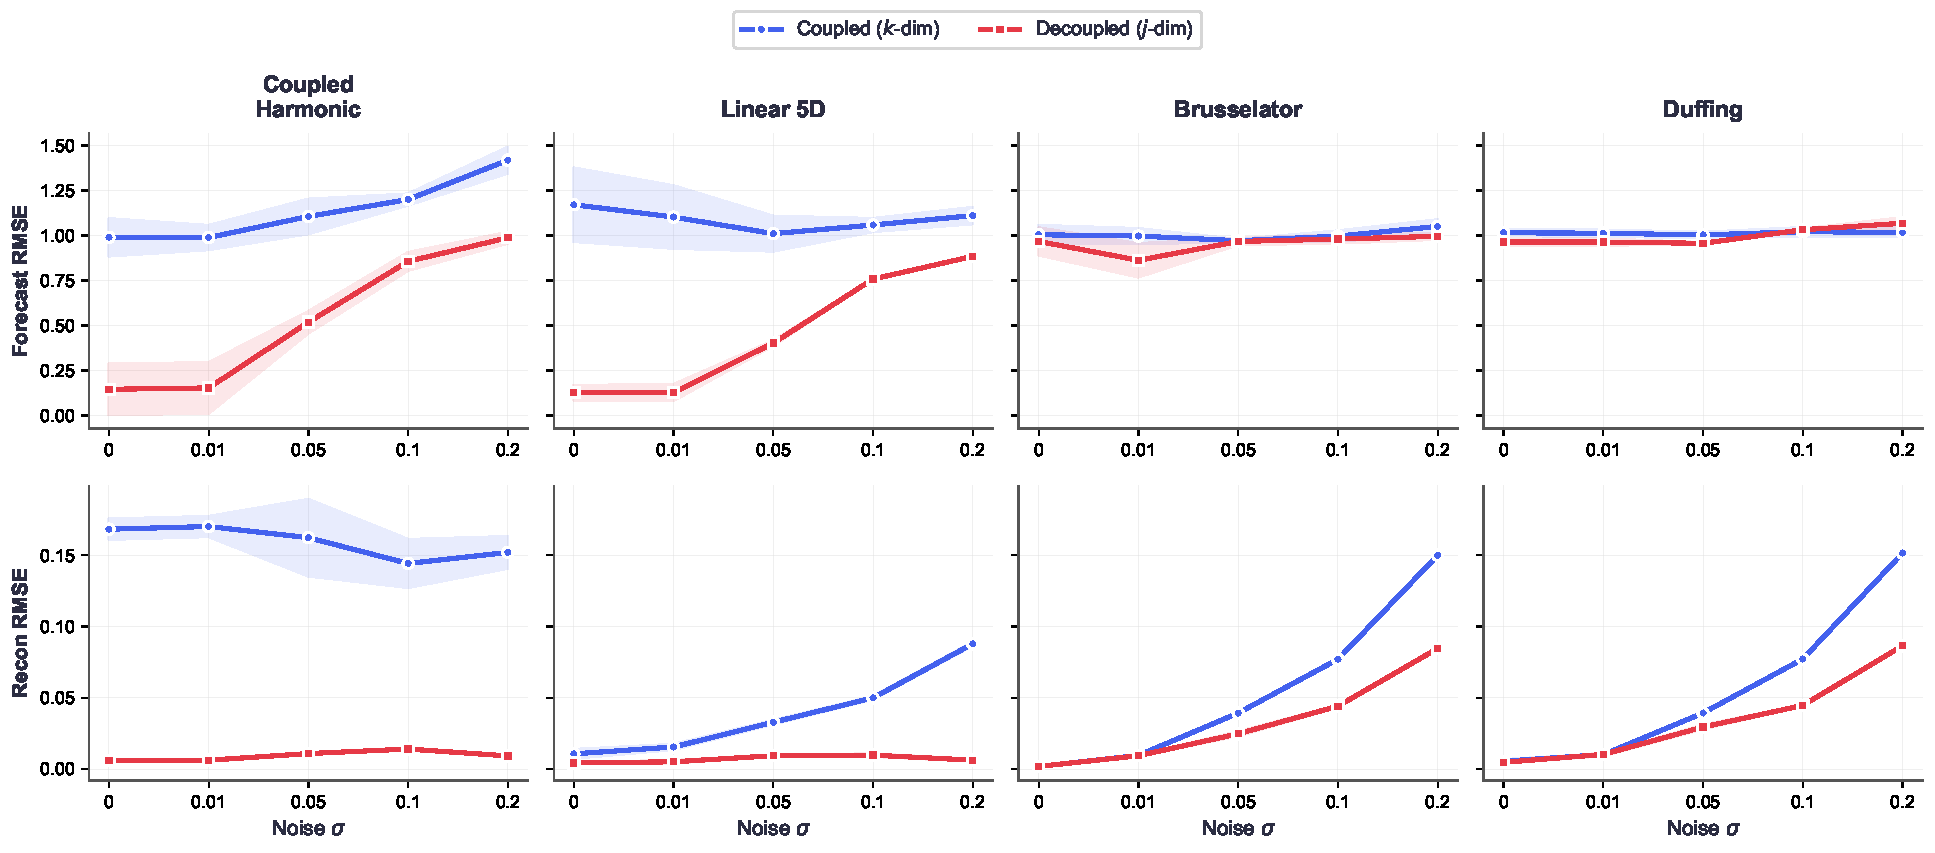
\includegraphics[width=\textwidth]{noise_sweep.png}
\caption{Noise degradation curves (500-step spectral DMD rollout).
Top: forecast RMSE; bottom: reconstruction RMSE.
Shaded bands: $\pm$1 std over 3 seeds.  Decoupled (red) maintains
lower error than Coupled (blue) across all noise levels on
Coupled Harmonic and Linear~5D; the two converge on the chaotic
systems at high noise.}
\label{fig:noise-sweep}
\end{figure}

\begin{table}[H]
\caption{DMD noise sensitivity: 500-step spectral rollout RMSE
(mean, 3 seeds).  \textbf{Bold}: best per cell.}
\label{tab:noise-dmd}
\centering
\small
\setlength{\tabcolsep}{2.5pt}
\begin{tabular}{l l ccccc}
\toprule
& & $\sigma{=}0$ & $\sigma{=}0.01$ & $\sigma{=}0.05$ & $\sigma{=}0.1$ & $\sigma{=}0.2$ \\
\midrule
\multirow{2}{*}{C.~Harm.}
  & Coupled   & .990 & .988 & 1.11 & 1.20 & 1.42 \\
  & Decoupled & $\mathbf{.146}$ & $\mathbf{.153}$ & $\mathbf{.518}$ & $\mathbf{.856}$ & $\mathbf{.988}$ \\
\addlinespace
\multirow{2}{*}{Lin.~5D}
  & Coupled   & 1.17 & 1.10 & 1.01 & 1.06 & 1.11 \\
  & Decoupled & $\mathbf{.127}$ & $\mathbf{.128}$ & $\mathbf{.402}$ & $\mathbf{.758}$ & $\mathbf{.884}$ \\
\addlinespace
\multirow{2}{*}{Bruss.}
  & Coupled   & 1.00 & $\mathbf{.997}$ & $\mathbf{.971}$ & $\mathbf{.996}$ & 1.05 \\
  & Decoupled & $\mathbf{.967}$ & $\mathbf{.862}$ & .967 & .980 & $\mathbf{.995}$ \\
\addlinespace
\multirow{2}{*}{Duffing}
  & Coupled   & 1.02 & 1.01 & 1.00 & $\mathbf{1.02}$ & $\mathbf{1.02}$ \\
  & Decoupled & $\mathbf{.964}$ & $\mathbf{.963}$ & $\mathbf{.957}$ & 1.03 & 1.07 \\
\bottomrule
\end{tabular}
\\[4pt]
{\footnotesize Forecast RMSE only; reconstruction RMSE visible in Figure~\ref{fig:noise-sweep}.}
\end{table}


% ======================================================================
\section{Discussion}
\label{sec:discussion}

The reconstruction--forecasting tradeoff arises when a single latent
must serve both objectives.  The capacity bound
(Proposition~\ref{prop:capacity}) shows that the optimal projections
for the two tasks generically differ; gradient conflict
(Proposition~\ref{prop:gradient-conflict}) shows that joint training
wastes optimiser effort through inter-task cancellation.

Carrier-residual decoupling addresses both: a wide carrier handles
reconstruction, a narrow residual code handles dynamics, and no
parameters are shared after Phase~1.  The ablation
(\S\ref{sec:ablation}) shows that no single frozen baseline achieves
what Decoupled provides.  The head comparison
(\S\ref{sec:head-comparison}) shows that no coupled variant---even
with a nonlinear ODE head---Pareto-dominates the decoupled model.
Multi-task gradient methods do not close the gap (\S\ref{sec:mtl}).
Three literature methods improve when run on the decoupled pipeline
(\S\ref{sec:literature}).

\paragraph{Limitations.}
The decoupled model adds parameters ($\psi$, $\mu$, GRU) beyond the
baseline AE; all coupled baselines are widened to match
($1.00$--$1.01\times$; Appendix~\ref{app:params}).  The three-phase
training is more involved than a single end-to-end pass.
Proposition~\ref{prop:capacity} is proved for linear systems and
extended to nonlinear ones via Corollary~\ref{cor:nonlinear}, but
the nonlinear bound relies on the Jacobian argument rather than a
direct global analysis.
All systems are synthetic.  On Lorenz-96 (chaotic), the advantage
is modest.

\paragraph{Future work.}
Extending decoupling to irregular time series, integrating it within
transformer-based temporal models, and developing rules for choosing
$j$ and $k$ are natural next steps.


% ======================================================================
\bibliographystyle{iclr2027_conference}
\bibliography{iclr2027}


% ======================================================================
\appendix

\section{Multi-Horizon Forecast}
\label{app:multi-horizon}

Table~\ref{tab:multi-horizon} evaluates forecast RMSE at horizons
$\tau \in \{1, 5, 10, 25, 50, 100\}$.  Coupled\_k is param-matched.
Decoupled tracks Frozen\_j closely at all horizons while the coupled
model degrades rapidly.

\begin{table}[H]
\caption{Multi-horizon forecast RMSE (mean, 5 seeds, spectral DMD).
Coupled\_k is param-matched.  \textbf{Bold}: best per row.}
\label{tab:multi-horizon}
\centering
\small
\setlength{\tabcolsep}{3pt}
\begin{tabular}{ll rrrrrr}
\toprule
System & Method & F1 & F5 & F10 & F25 & F50 & F100 \\
\midrule
\multirow{3}{*}{C.~Harm.}
  & Coupled\_k & .715 & .735 & .786 & .960 & 1.20 & 1.40 \\
  & Frozen\_j  & .007 & .022 & .040 & .069 & .085 & .088 \\
  & Decoupled  & \textbf{.007} & \textbf{.022} & \textbf{.039} & \textbf{.068} & \textbf{.083} & \textbf{.086} \\
\addlinespace
\multirow{3}{*}{Lin.~5D}
  & Coupled\_k & .574 & .590 & .667 & .900 & 1.26 & 1.73 \\
  & Frozen\_j  & \textbf{.006} & \textbf{.018} & \textbf{.033} & \textbf{.064} & \textbf{.091} & \textbf{.095} \\
  & Decoupled  & .006 & .018 & .033 & .065 & .092 & .098 \\
\addlinespace
\multirow{3}{*}{Bruss.}
  & Coupled\_k & .467 & .609 & .899 & 1.33 & 1.67 & 1.54 \\
  & Frozen\_j  & .009 & .036 & .159 & .501 & \textbf{.801} & \textbf{.726} \\
  & Decoupled  & \textbf{.008} & \textbf{.035} & \textbf{.157} & \textbf{.497} & .803 & .736 \\
\addlinespace
\multirow{3}{*}{Duffing}
  & Coupled\_k & .506 & .532 & .623 & .890 & 1.53 & 2.63 \\
  & Frozen\_j  & .006 & \textbf{.010} & \textbf{.050} & .340 & .744 & 1.10 \\
  & Decoupled  & \textbf{.005} & .011 & .052 & \textbf{.338} & \textbf{.735} & \textbf{1.09} \\
\addlinespace
\multirow{3}{*}{L-96}
  & Coupled\_k & .701 & .854 & .931 & 1.00 & 1.00 & 1.05 \\
  & Frozen\_j  & \textbf{.420} & .815 & 1.03 & 1.18 & \textbf{1.29} & 1.25 \\
  & Decoupled  & .420 & \textbf{.812} & \textbf{1.03} & \textbf{1.18} & 1.30 & \textbf{1.25} \\
\bottomrule
\end{tabular}
\end{table}


\section{Training Details and Reproducibility}
\label{app:training}

All models use 2-hidden-layer MLPs with ELU activations and hidden
width $h{=}64$.  Training: Adam, $\mathrm{lr}{=}10^{-3}$, batch 512,
400 epochs/phase.  Seeds: $\{0,1,2,42,123\}$ (noise: $\{0,1,42\}$).

Phase~1 trains $E{+}D$.  Phase~2 freezes $E{+}D$, trains $\psi{+}\mu$.
Phase~3 freezes all but the GRU.  DMD is fitted post-hoc.

Coupled MLP and ODE heads are trained jointly at $\varphi{=}0.5$ with
gradient clipping ($\mathrm{max\_norm}{=}1$).
Decoupled heads are trained on the frozen $b$ trajectory (Phase~2.5).

\paragraph{Parameter matching.}\label{app:params}
Each coupled baseline uses a wider hidden layer $h$ so its param
count $\ge$ the decoupled model's (Table~\ref{tab:paramcounts}).

\begin{table}[H]
\centering\small
\caption{Parameter counts.}
\label{tab:paramcounts}
\begin{tabular}{lccccc}
\toprule
System & $n$ & Coupled $h$ & Coupled & Decoupled & Ratio \\
\midrule
C.~Harmonic & 6  & 73 & 12\,436 & 12\,362 & 1.01$\times$ \\
Linear 5D   & 5  & 73 & 12\,289 & 12\,233 & 1.00$\times$ \\
Brusselator & 10 & 73 & 12\,870 & 12\,749 & 1.01$\times$ \\
Duffing     & 10 & 73 & 12\,870 & 12\,749 & 1.01$\times$ \\
Lorenz-96   & 20 & 76 & 16\,546 & 16\,478 & 1.00$\times$ \\
KS-64D      & 64 & 95 & 33\,966 & 33\,488 & 1.01$\times$ \\
\bottomrule
\end{tabular}
\end{table}
\noindent
Latent dimensions: C.~Harmonic ($k{=}4$, $j{=}8$),
Linear~5D ($k{=}4$, $j{=}8$), Brusselator ($k{=}3$, $j{=}8$),
Duffing ($k{=}3$, $j{=}8$), L-96 ($k{=}10$, $j{=}12$),
KS-64D ($k{=}16$, $j{=}32$).

\paragraph{Data generation.}
All systems: \texttt{solve\_ivp} (RK45, $\mathrm{rtol}{=}\mathrm{atol}{=}10^{-10}$,
$\Delta t{=}0.05$, $[0,500]$ time units).  First 200 samples
discarded.  Train: 4000 samples; test: 500.


\section{AI Assistance and Formal Verification}
\label{app:ai-disclosure}

This work used Claude (Anthropic) as a writing aid.  All
experimental code, theory, architecture, and scientific claims are
the author's sole work.

Both propositions and the nonlinear corollary have been formally
verified in Lean~4 using the Mathlib library.  The proof assistant's
kernel machine-checks every deduction against its type theory,
providing a certificate of logical validity independent of human
review.  The formalisation source is included in the supplementary
material.


\end{document}
